\documentclass[11pt,a4paper]{article}

\usepackage[utf8]{inputenc}
\usepackage[T1]{fontenc}
\usepackage{amsmath, amssymb, amsthm}
\usepackage{booktabs}
\usepackage{graphicx}
\usepackage{hyperref}
\usepackage{xcolor}
\usepackage{algorithm}
\usepackage{algpseudocode}
\usepackage{multirow}
\usepackage{geometry}
\usepackage{natbib}
\usepackage{caption}
\usepackage{subcaption}
\usepackage{enumitem}

\geometry{margin=1in}

\hypersetup{
    colorlinks=true,
    linkcolor=blue!60!black,
    citecolor=blue!60!black,
    urlcolor=blue!60!black
}

\newtheorem{definition}{Definition}
\newtheorem{proposition}{Proposition}

\title{
    \vspace{-1cm}
    \textbf{Metric Selection for the Objective Evaluation\\
    of System Prompts in Large Language Models}\\
    \vspace{0.4cm}
    \large Distributional Signals, Programmatic Verification,\\
    and Structured Judgment as Evaluation Foundations
}

\author{
    Axel Fritz\\
    \texttt{axel.fritz@alquimia.ai}\\
    Alquimia AI
    \and
    Alex Fiorenza\\
    \texttt{alex.fiorenza@alquimia.ai}\\
    Alquimia AI
}

\date{March 30, 2026}

% ─────────────────────────────────────────────────────────────────────────────

\begin{document}

\maketitle

\begin{abstract}
Evaluating the quality of a system prompt for a large language model (LLM) is a non-trivial task. Existing approaches often collapse quality into a single scalar score derived from a single LLM judge call, which lacks scientific grounding and diagnostic value. In this work, we analyze the space of available metrics for prompt evaluation and propose a set of components with distinct root causes, organized by objectivity and availability. Our main proposal for integration in evaluation libraries is grounded in two objective and reproducible metrics as a mandatory core: the Consistency/Stability Rate (CSR), which measures how stable the model's response distribution is under repeated sampling, and the normalized Semantic Entropy (SE), which quantifies uncertainty over the space of meanings of the outputs. Three optional components are added, which the user can enable according to their use case: the Reference Similarity Score (RSS), applicable when reference responses are available, the Instruction Compliance Rate (ICR), applicable when the prompt contains programmatically verifiable constraints, and the Judge Quality (JQ), for those who prioritize exhaustiveness over strict reproducibility. This design decision—privileging objectivity and reproducibility in the core, delegating to the user the incorporation of signals dependent on external models—is formally justified throughout the paper.
\end{abstract}

% ─────────────────────────────────────────────────────────────────────────────
\section{Introduction}
% ─────────────────────────────────────────────────────────────────────────────

The quality of a system prompt has a direct impact on the behavior of an LLM in production. Yet, despite the central role of prompt engineering in applied AI, rigorous methods for prompt evaluation remain underexplored. Most practitioners rely on anecdotal comparisons or single-call LLM judges that produce a score with no explicit scientific justification.

This paper addresses the following question: \textit{What is a scientifically defensible way to score a system prompt, and what should that score represent?}

Our answer is grounded in three observations from the literature. First, a single score is difficult to defend unless the dimensions it aggregates are made explicit \citep{unieval2022}. Second, high output consistency under sampling is a meaningful distributional signal of prompt quality, but consistency alone does not imply correctness \citep{selfconsistency2023, glape2024}. Third, multi-objective reward models trained on human preference data outperform single-score LLM judges on standard benchmarks, and their advantage lies precisely in operating over a vector of objectives \citep{armorm2024}.

We propose to return a vector $\mathbf{m}$ of five normalized signals organized in two tiers. The mandatory core consists of two reference-free distributional metrics: the Consistency/Stability Rate (CSR) \citep{selfconsistency2023, glape2024}, which measures how often the model produces semantically equivalent responses under repeated sampling, and normalized Semantic Entropy (SE) \citep{semanticentropy2024}, which quantifies uncertainty over the space of meanings. Three optional signals extend the core when dependencies are available: Reference Similarity Score (RSS), Instruction Compliance Rate (ICR) \citep{ifeval2023}, and Judge Quality (JQ). Scalar aggregation is left as an optional, explicitly calibrated step.

The central empirical finding of this work is that \textbf{no single signal is sufficient for behavioral prompt evaluation}. In a controlled experiment comparing a well-specified, a deliberately wrong, and a minimal system prompt for a customer service bot, we show that:
\begin{itemize}[noitemsep]
    \item CSR and Stability correctly order all three prompts by behavioral consistency but cannot detect \textit{what} the model is doing wrong.
    \item RSS cannot distinguish a prompt that follows the \textit{wrong} protocol (JQ = 0.200) from one that provides \textit{no} protocol at all (JQ = 0.500)---their embedding distances from the reference are nearly identical (0.599 vs.\ 0.617).
    \item ICR detects constraint non-compliance with certainty but only for constraints that were explicitly defined.
    \item JQ is the only signal that exposes active protocol violation: the wrong-instruction prompt scores \textit{below} the minimal prompt because the model consistently follows bad instructions rather than improvising.
\end{itemize}
These results justify the compound vector design: each signal exposes a failure mode that the others miss.

% ─────────────────────────────────────────────────────────────────────────────
\section{Related Work}
% ─────────────────────────────────────────────────────────────────────────────

\paragraph{Self-consistency and distributional signals.}
\citet{selfconsistency2023} propose self-consistency as a decoding strategy: multiple reasoning chains are sampled and the most frequent answer is selected via majority vote. This establishes output frequency as a reference-free signal of model stability. \citet{glape2024} extend this to prompt evaluation, defining self-consistency as the mode frequency among $n$ sampled outputs and introducing a mutual-consistency refinement across prompt variants. They report Spearman correlation with ground-truth accuracy and show that GLaPE outperforms raw self-consistency across eight reasoning datasets.

\paragraph{Programmatic instruction verification.}
\citet{ifeval2023} propose IFEval, which restricts evaluation to verifiable instructions—those whose compliance can be checked with a deterministic program (e.g., word count, JSON format, keyword inclusion). They define strict and loose compliance metrics at both the prompt and instruction level, providing a reproducible and objective evaluation component.

\paragraph{Prompt perplexity.}
\citet{promptperplexity2022} show that prompts with lower perplexity tend to yield better task performance, interpreting perplexity as a proxy for model familiarity with the prompt. They propose SPELL, a method to select and expand prompt candidates by ranking on perplexity over a held-out sample of inputs.

\paragraph{Multi-dimensional evaluation.}
\citet{unieval2022} argue that human evaluation of natural language generation (NLG) is inherently multi-dimensional (e.g., coherence, fluency, relevance) and that a one-size-fits-all score is scientifically untenable. They reformulate each dimension as a Boolean question answered by a unified model, reporting probabilities of ``Yes'' as dimension-level scores.

\paragraph{Reward models.}
\citet{rewardbench2024} formalize reward model evaluation using triples (prompt, chosen, rejected) and define accuracy as the rate at which the model assigns a higher score to chosen over rejected. \citet{armorm2024} extend this to multi-objective reward modeling: a vector of absolute ratings is predicted and dynamically scalarized via a gating network conditioned on the prompt, arguing that fixed-weight linear combinations are too rigid for general use.

\paragraph{LLM-as-a-judge.}
\citet{geval2023} propose G-Eval, which uses chain-of-thought followed by structured form-filling to evaluate NLG dimensions, reporting Spearman correlation of 0.514 with human judgments in summarization. They also document systematic biases in LLM judges, including position bias and preference for LLM-generated text.

% ─────────────────────────────────────────────────────────────────────────────
\section{Method}
% ─────────────────────────────────────────────────────────────────────────────

\subsection{Notation and Sampling Setup}

The central idea of the method is not to evaluate the prompt with a single model response, but to observe how the model behaves when asked the same question multiple times. We call $p$ the prompt under evaluation, $x$ an input query, and $K$ the number of times the model generates a response for each pair $(p, x)$.

Formally, $\{y_k\}_{k=1}^{K}$ are the $K$ outputs generated with temperature $T > 0$ (which introduces variability between responses) and $\mathcal{D} = \{x_j\}_{j=1}^{J}$ is the set of queries over which the prompt is evaluated. The result per instance is a vector $\mathbf{m}(p, x)$; the global prompt result is the average over all queries:
\[
\bar{\mathbf{m}}(p) = \frac{1}{J} \sum_{j=1}^{J} \mathbf{m}(p, x_j)
\]

\subsection{Tier 1 — Core Metrics (Always Applicable)}

Tier 1 consists of two components that require no special infrastructure: only $K$ model calls. They work with any prompt, any provider, and any dataset.

\subsubsection{CSR — Consistency/Stability Rate}

A quality prompt should lead the model to give coherent responses to each other, even when run multiple times with positive temperature. CSR measures exactly that: what fraction of the $K$ responses falls into the most frequent group.

If we run the same prompt 10 times and 7 responses say essentially the same thing, then CSR = 0.70. A prompt that produces scattered and contradictory responses will have low CSR.

Formally, let $a_k$ be the response extracted from sample $k$ (via regex for numeric QA, or semantic grouping for free text). Following \citet{selfconsistency2023} and \citet{glape2024}:

\begin{definition}[CSR]
\[
\mathrm{CSR}(p, x) = \max_{a} \frac{1}{K} \sum_{k=1}^{K} \mathbf{1}[a_k = a]
\]
\end{definition}

For free text, responses are grouped semantically (see \S\ref{sec:clustering}) and CSR is the mass of the largest cluster: $\max_{\ell} n_\ell / K$, where $n_\ell$ is the number of responses in cluster $\ell$. CSR $\in [0, 1]$ by construction.

\subsubsection{SE — Semantic Entropy}

CSR only looks at the most frequent group. SE complements that view by measuring the complete distribution of meanings: if responses cluster into a few very dense groups, entropy is low (the model is certain). If they scatter into many different groups, entropy is high (the model is uncertain).

The key difference from token entropy is that SE groups first by meaning, not by form. Two responses that say the same thing with different words count as one \citep{semanticentropy2024}.

Let $\{C_\ell\}$ be the semantic clusters of the $K$ responses, with $n_\ell$ responses each. In the discrete variant (without needing to access internal model probabilities):
\[
\hat{p}(C_\ell \mid x) = \frac{n_\ell}{K}, \qquad
\mathrm{SE}(p, x) = -\sum_{\ell} \hat{p}(C_\ell \mid x) \log \hat{p}(C_\ell \mid x)
\]

We normalize by $\log K$ so the result falls in $[0, 1]$, and invert it so that a higher score is better. This normalization requires $K \geq 2$; in the degenerate case $K = 1$ we define $\mathrm{SE}_n(p, x) = 0$ by convention:
\[
\mathrm{SE}_n(p, x) = \frac{\mathrm{SE}(p, x)}{\log K}, \qquad \text{component in } \mathbf{m}: \ 1 - \mathrm{SE}_n
\]

\subsection{Semantic Clustering Strategy}
\label{sec:clustering}

Both CSR and SE depend on being able to group the $K$ responses by semantic equivalence. There are two approaches for determining whether two responses belong to the same cluster:

\begin{itemize}[noitemsep]
    \item \textbf{Bidirectional NLI}: two responses are grouped if a natural language inference model verifies that $y_i \Rightarrow y_j$ and $y_j \Rightarrow y_i$. This is the most rigorous method but requires an additional NLI model and has $O(K^2)$ cost in calls.
    \item \textbf{Cosine similarity over embeddings}: we construct an undirected graph on the $K$ responses with an edge between $y_i$ and $y_j$ if $\mathrm{cos}(\mathbf{e}_i, \mathbf{e}_j) \geq \tau$, where $\mathbf{e}_i$ is the embedding of response $y_i$ and $\tau$ is a configurable threshold, and define clusters as the connected components of this threshold graph (equivalently, single-linkage clustering with similarity threshold $\tau$).
\end{itemize}

We adopt cosine similarity with connected-components over the threshold graph as the clustering strategy for three reasons: it requires no additional model beyond the embedding model already available in the system, the threshold $\tau$ is explicit and configurable by the user, and the cost is significantly lower than NLI.

\paragraph{Effect of threshold $\tau$.}
The threshold determines how similar two responses must be to be considered equivalent. Table~\ref{tab:tau} describes the effect on CSR and SE according to the value of $\tau$.

\begin{table}[h]
\centering
\caption{Effect of threshold $\tau$ on CSR and SE.}
\label{tab:tau}
\begin{tabular}{p{2cm} p{3.5cm} p{3.5cm} p{3.5cm}}
\toprule
Value of $\tau$ & Behavior & Effect on CSR and SE & When to use \\
\midrule
$\tau < 0.70$ &
Very permissive. Groups superficially similar responses even if they say different things. &
Artificially high CSR. Artificially low SE. Overestimates prompt consistency. &
Not recommended. \\
\addlinespace
$\tau = 0.75$--$0.85$ &
Balanced. Groups paraphrases and style variations; separates responses with different content. &
Representative estimates of the prompt's real behavior. &
Recommended default configuration. \\
\addlinespace
$\tau = 0.85$--$0.92$ &
Strict. Only groups nearly identical responses in content and phrasing. &
Lower CSR, higher SE. Detects subtle content variations. &
High-precision evaluations or prompts with highly structured responses. \\
\addlinespace
$\tau > 0.92$ &
Very strict. Almost all responses fall into different clusters. &
CSR and SE lose diagnostic value — every superficial variation is interpreted as semantic. &
Not recommended except for very specific cases. \\
\bottomrule
\end{tabular}
\end{table}

\noindent The recommended default value is $\tau = 0.90$ for sentence-transformer embedders in the 22M--110M parameter range (see \S\ref{sec:experiments} for empirical justification). Users in domains with high style variability (e.g., conversational responses) can reduce it toward $0.80$; values above $0.92$ are not recommended.

\subsection{Tier 2 — Extended Metrics (Conditional on Dependencies)}

These components increase the precision of the vector but require dependencies that are not always available. They are included in $\mathbf{m}$ only when applicable.

\subsubsection{RSS — Reference Similarity Score}

CSR and SE measure distributional stability but do not indicate whether the responses are correct. When reference responses are available, RSS provides an objective correctness signal without introducing the variance of an external judge model.

RSS computes the average cosine similarity between each generated response and the reference response $y^*$, using the same embedding model already used for clustering:

\begin{definition}[RSS]
\[
\mathrm{RSS}(p, x) = \frac{1}{K} \sum_{k=1}^{K} \mathrm{cos}\!\left(\mathbf{e}(y_k),\, \mathbf{e}(y^*)\right)
\]
\end{definition}

\noindent where $\mathbf{e}(\cdot)$ denotes the embedding of a response. RSS $\in [-1, 1]$ by construction; in practice it falls in $[0, 1]$ for semantically related texts.

Unlike JQ, RSS does not depend on an LLM judge and produces the same result given the same embedder, dataset, and prompt. Its limitation is that embedding similarity captures surface-level semantic proximity but may not detect factual errors that are semantically close to the reference.

\subsubsection{ICR — Instruction Compliance Rate}

Some prompts include instructions that can be verified with a program, without needing a judge: ``respond in JSON'', ``use fewer than 100 words'', ``include keyword X''. ICR measures what fraction of those constraints are met, deterministically and reproducibly \citep{ifeval2023}.

If the prompt has 3 verifiable constraints and the response meets 2, $\mathrm{ICR}_\mathrm{inst} = 0.67$. If none are met, $\mathrm{ICR}_\mathrm{prompt} = 0$ and it can be used as a hard gate: the output is rejected regardless of other scores.

\begin{definition}[ICR]
\[
\mathrm{ICR}_\mathrm{inst}(p, x) = \frac{1}{KM} \sum_{k=1}^{K} \sum_{m=1}^{M} \mathbf{1}\left[\mathrm{is\_followed}(y_k, c_m)\right]
\qquad
\mathrm{ICR}_\mathrm{prompt}(p, x) = \frac{1}{K} \sum_{k=1}^{K} \mathbf{1}\left[\bigwedge_{m=1}^{M} \mathrm{is\_followed}(y_k, c_m)\right]
\]
\end{definition}

\subsubsection{JQ — Judge Quality (Multi-Rubric)}

CSR and SE measure distributional stability, but do not say whether the responses are \textit{good}. For that we use an LLM judge, but with an important difference from a naïve judge: instead of asking for a single number, we ask it to evaluate the response on four independent dimensions and return a structured JSON.

This forces the judge to reason step by step (chain-of-thought) before assigning each sub-score, reducing the arbitrariness of a single score \citep{geval2023, unieval2022}.

The final JQ score is the average of the four sub-scores $s_d \in [0,1]$:

\begin{definition}[JQ]
\[
\mathrm{JQ}(p, x) = \frac{1}{D} \sum_{d=1}^{D} s_d
\]
\end{definition}

\begin{table}[h]
\centering
\caption{Rubric dimensions for JQ.}
\begin{tabular}{lll}
\toprule
Dimension & Symbol & What it measures \\
\midrule
Utility / Completeness & $s_1$ & Does the response answer the query? \\
Faithfulness to context & $s_2$ & No hallucination beyond provided context \\
Instruction adherence & $s_3$ & Follows non-verifiable prompt directives \\
Clarity & $s_4$ & Coherent, well-structured response \\
\bottomrule
\end{tabular}
\end{table}

\noindent \textbf{Bias mitigation:} To reduce position bias documented in LLM judges \citep{geval2023}, the evaluation is repeated $R \geq 3$ times with randomized output ordering and results are averaged.


\subsection{The Metric Vector}

The final result of evaluating a prompt $p$ over a query $x$ is the vector $\mathbf{m}$, where each component has a distinct root cause and all are normalized to $[0, 1]$:

\begin{definition}[Metric vector]
\[
\mathbf{m} = \left[\mathrm{CSR},\ 1 - \mathrm{SE}_n,\ \underbrace{\mathrm{RSS}^*,\ \mathrm{ICR}^*,\ \mathrm{JQ}^*}_{\text{optional}}\right]
\]
\end{definition}

\noindent where ${}^*$ indicates components included only when their dependencies are available.

% ─────────────────────────────────────────────────────────────────────────────
\section{Experiments}
\label{sec:experiments}
% ─────────────────────────────────────────────────────────────────────────────

We evaluate the proposed metric vector on a behavioral benchmark for a customer service assistant. Unlike factual domains---where capable models tend to produce semantically convergent responses regardless of prompt quality---behavioral queries expose prompt quality directly: the correct action (escalation protocol, off-topic redirect, incomplete-input handling) is an arbitrary policy prescribed only by the prompt, and without that policy capable models produce diverse but plausible responses, creating observable variance in all signals.

\subsection{Experimental Setup}

\textbf{Model and embedder.} We use \texttt{qwen/qwen3-32b} via the Groq API with temperature $T = 0.7$ and \texttt{reasoning\_effort=none} to suppress chain-of-thought output that would otherwise contaminate embedding similarity scores (see \S\ref{sec:tau_k}). Embeddings are computed with \texttt{all-MiniLM-L6-v2} (22M parameters). All experiments use $K = 10$ samples per query and $\tau = 0.90$.

\textbf{Dataset.} The evaluation dataset consists of $J = 10$ behavioral queries for a WhatsApp customer service assistant of a Japanese restaurant. Queries cover: three complaints (incorrect order, cold food, delivery delay), two off-topic redirects (competitor recommendation, movie recommendation), one health/safety query (possible food poisoning), two incomplete reservation requests (missing time, missing party size), one discount negotiation, and one aggressive message. All ground-truth reference responses reflect the protocol prescribed by the good prompt.

\textbf{Prompt variants.} Three system prompt variants are evaluated:
\begin{itemize}[noitemsep]
    \item \textit{Good}: eight explicit behavioral instructions specifying complaint escalation to the \textit{encargado} (manager), off-topic redirect without answering, incomplete reservation validation (must request all missing data before confirming), health/safety protocol (refer to medical professional and escalate), de-escalation for aggressive messages, and correct discount policy.
    \item \textit{Bad}: six explicitly wrong instructions that contradict the correct protocol---resolve complaints directly without escalation, grant any requested discount, confirm reservations without requesting missing data, provide home remedies for food poisoning, and engage freely with off-topic queries.
    \item \textit{Simple}: a minimal prompt providing only role identification (124 characters), with no behavioral instructions.
\end{itemize}

\textbf{Signals.} All five components of $\mathbf{m}$ are activated: CSR and Stability (mandatory core); RSS with ground-truth reference responses; ICR with a single \texttt{KeywordConstraint} checking for the escalation keyword \textit{encargado} (mandated by the good prompt in five query types); and JQ with a behavioral rubric objective specifying the correct customer service protocol.

\subsection{Why Behavioral Queries}

Factual queries have a single semantically convergent correct answer derivable from model training. Behavioral queries---complaints, off-topic requests, incomplete inputs---are genuinely ambiguous: a polite, helpful response can take many valid forms. The correct action is an arbitrary policy prescribed only by the prompt. Without that policy, capable models produce diverse but plausible responses, creating observable variance in CSR and Stability. A bad prompt can actively prescribe the wrong policy, producing consistent but incorrect behavior---the failure mode that motivates the multi-signal design.

\subsection{Results}

Table~\ref{tab:results} reports the mean metric vector per prompt variant averaged over all $J = 10$ queries.

\begin{table}[h]
\centering
\caption{Mean metric vector per prompt variant ($K=10$, $\tau=0.90$, $T=0.7$, \texttt{qwen/qwen3-32b}). Stability $= 1 - \mathrm{SE}_n$.}
\label{tab:results}
\begin{tabular}{lccccc}
\toprule
Prompt & CSR & Stability ($1-\mathrm{SE}_n$) & RSS & ICR & JQ \\
\midrule
Good   & 0.400 & 0.301 & 0.702 & 1.000 & 0.875 \\
Bad    & 0.200 & 0.060 & 0.599 & 0.000 & 0.200 \\
Simple & 0.100 & 0.000 & 0.617 & 0.000 & 0.500 \\
\bottomrule
\end{tabular}
\end{table}

\begin{figure}[h]
\centering
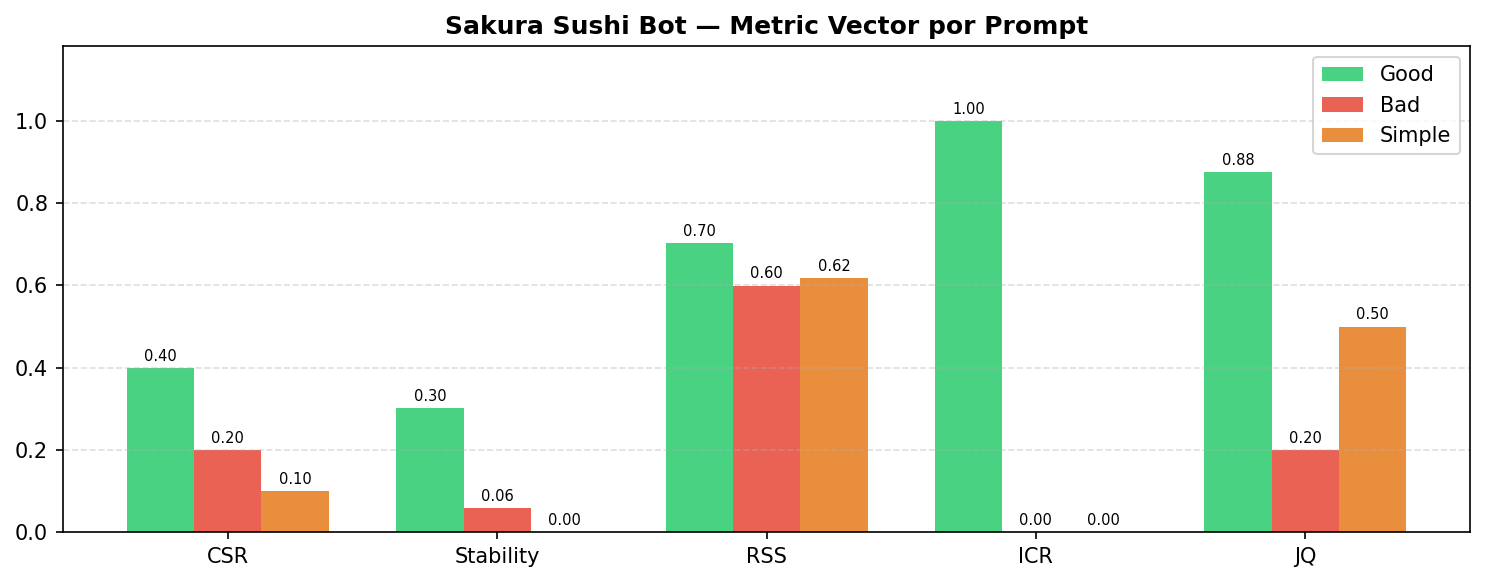
\includegraphics[width=0.72\textwidth]{figures/sushi_bar_overall.png}
\caption{Metric vector per prompt variant ($K=10$, $\tau=0.90$, $T=0.7$). Each bar group corresponds to one signal; colors indicate prompt quality (green = good, red = bad, orange = simple).}
\label{fig:bar}
\end{figure}

\begin{figure}[h]
\centering
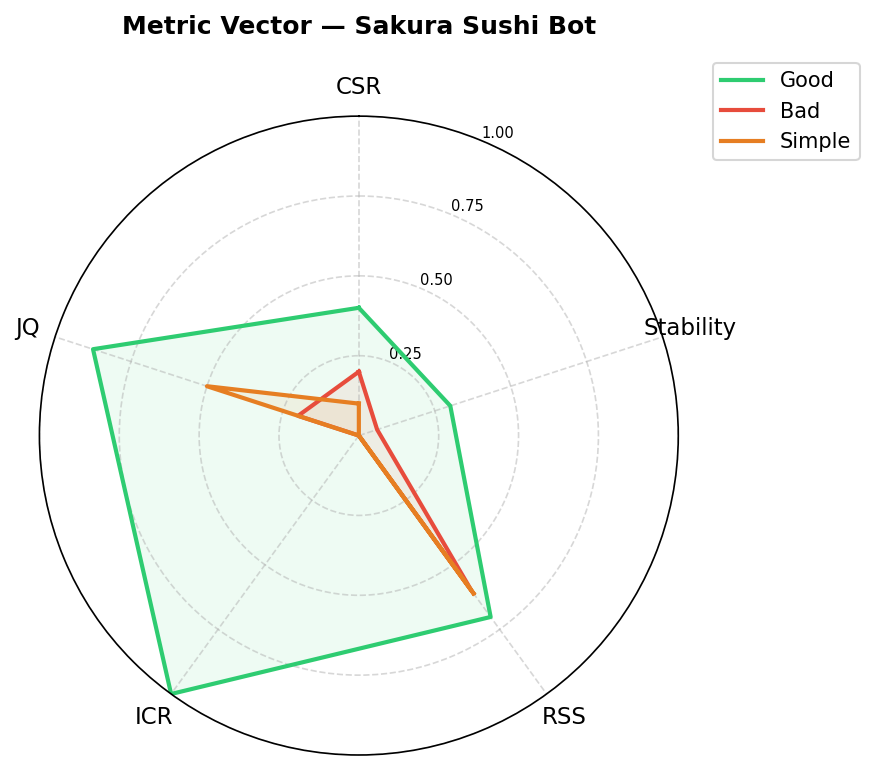
\includegraphics[width=0.48\textwidth]{figures/sushi_radar.png}
\caption{Radar chart of the full metric vector per prompt variant. The good prompt (green) fills the polygon across all five signals; the bad and simple prompts show distinct collapse patterns revealing different failure modes.}
\label{fig:radar}
\end{figure}

\subsection{Analysis}

\paragraph{CSR and Stability: behavioral instructions enforce consistent behavior.}
All three variants are correctly ordered: Good (CSR = 0.400, Stability = 0.301) $>$ Bad (0.200, 0.060) $>$ Simple (0.100, 0.000). Absolute CSR values are lower than typical factual evaluations because behavioral queries are genuinely multi-valid in the absence of explicit instructions---even a good prompt cannot fully eliminate semantic variation across $K$ samples. The simple prompt achieves minimum Stability ($= 0.000$): the model improvises a different behavioral approach on almost every sample, producing maximum semantic entropy.

\paragraph{RSS alone cannot distinguish bad from simple.}
RSS scores: Good = 0.702, Simple = 0.617, Bad = 0.599. The good prompt is correctly identified as the best by RSS, but bad and simple are nearly indistinguishable---and their ordering is inverted (simple $>$ bad). The explanation is that embedding-based similarity captures topic-level semantics: a response that tries to resolve a complaint directly and one that escalates to the manager both discuss the complaint domain and embed similarly relative to the reference. RSS is insufficient as a sole discriminator when prompt failures consist of following the wrong protocol rather than going off-topic.

\paragraph{ICR produces perfect binary separation.}
ICR drops from 1.000 (Good) to 0.000 for both Bad and Simple---a perfect binary separation. The good prompt always invokes the escalation keyword \textit{encargado} in the five relevant query types; the bad prompt explicitly instructs against escalation and the simple prompt provides no protocol. This illustrates the value of ICR as a deterministic gate: when a constraint is defined, its violation is detected with certainty and without judge variance.

\paragraph{JQ reveals active protocol violation in the bad prompt.}
The critical multi-signal finding is the gap between Bad (JQ = 0.200) and Simple (JQ = 0.500). RSS inverts this ordering; JQ corrects it. The bad prompt actively instructs the model to violate the correct protocol---offering direct refunds for complaints, providing home remedies for food poisoning, confirming incomplete reservations without requesting missing data---and the model follows these wrong instructions consistently. The simple prompt, by contrast, produces improvised responses that are sometimes acceptable for straightforward queries, yielding a higher JQ on average. This is the ``consistently wrong'' pattern at the protocol level: consistent behavior (CSR = 0.200) with systematically incorrect responses, a failure invisible to RSS but exposed by JQ.

\paragraph{No single signal is sufficient.}
Table~\ref{tab:failures} summarizes the failure modes exposed exclusively by each signal.

\begin{table}[h]
\centering
\caption{Failure modes exposed by each signal in the behavioral evaluation.}
\label{tab:failures}
\begin{tabular}{lp{8.5cm}}
\toprule
Signal & Failure it exposes \\
\midrule
CSR / Stability & Behavioral inconsistency: simple prompt improvises every time \\
RSS             & Semantic drift from reference behavior (good vs.\ others); insufficient for protocol violation \\
ICR             & Constraint non-compliance: escalation keyword never invoked by bad or simple \\
JQ              & Active protocol violation in bad prompt; invisible to RSS and ICR alone \\
\bottomrule
\end{tabular}
\end{table}

\noindent No signal in isolation correctly ranks all three prompt variants or exposes all failure modes. The compound metric vector is necessary for complete diagnostic coverage.

\subsection{Effect of $\tau$ and $K$}
\label{sec:tau_k}

We conducted a calibration analysis to characterize the sensitivity of CSR and Stability to the threshold $\tau$. With $\tau = 0.80$ and $K = 10$, over 90\% of queries produced $n_\mathrm{clusters} = 1$, saturating CSR at 1.0 across all prompt variants and eliminating discriminative value. The root cause is that \texttt{all-MiniLM-L6-v2} places factually similar responses at cosine similarity above 0.80 regardless of surface-level variation. Raising $\tau$ to 0.90 restores non-trivial cluster structure.

A secondary analysis over the grid $\tau \in \{0.80, 0.85, 0.90, 0.95\}$ and $T \in \{0.7, 0.9, 1.1\}$ (fixed prompt: behavioral good, $K = 5$) showed that temperature has a limited effect on CSR: the range across $T = 0.7$--$1.1$ for a fixed $\tau$ is at most $\pm 0.05$. The main sensitivity lever is $\tau$. These results justify $\tau = 0.90$ as the recommended default for sentence-transformer embedders in the 22M--110M parameter range, and confirm that the metric is robust to typical variation in user-configured temperature.

An additional implementation consideration arises with chain-of-thought models: \texttt{qwen/qwen3-32b} emits \texttt{<think>...</think>} blocks before the actual response. These reasoning tokens, when included in the embedded text, make every response semantically unique---collapsing CSR and Stability to their minimum values regardless of actual behavioral consistency. Disabling thinking mode (or stripping reasoning tokens before embedding) is required when evaluating models with chain-of-thought output. Similarly, when a \texttt{context} field provides domain knowledge accessible to both prompt variants under evaluation, the information asymmetry the experiment is designed to test is eliminated; domain knowledge must be embedded exclusively in the prompt under evaluation, not in a shared context.

% ─────────────────────────────────────────────────────────────────────────────
\section{Discussion and Limitations}
\label{sec:discussion}
% ─────────────────────────────────────────────────────────────────────────────

\paragraph{Why a vector, not a scalar.}
Three independent lines of evidence support returning $\mathbf{m}$ as the primary output. UniEval \citep{unieval2022} shows that human evaluation of NLG is multi-dimensional and that a unified evaluator must be explicitly designed around those dimensions. GLaPE \citep{glape2024} demonstrates quantitatively that a single signal (SC) can correlate poorly with accuracy. ArmoRM \citep{armorm2024} formally argues that fixed-weight linear scalarization of multiple objectives is too rigid, and that context-dependent weighting is required for a scalar to be principled.

\paragraph{Limitations.}
Tier 2 components introduce dependencies (logprob access, NLI model, reward model) that are not available in all deployment settings. ICR requires that the prompt contain programmatically verifiable constraints, which is not universally the case. Calibration of $S$ requires a set of human annotations or reference labels. RSS captures topic-level semantic proximity but cannot detect protocol-level failures: responses that follow the wrong behavioral protocol and responses that improvise freely can embed at similar distances from the reference, making RSS insufficient to distinguish them. For behavioral evaluation, JQ is the primary signal for detecting protocol violation.

\paragraph{Consistent incorrectness.}
CSR and SE measure distributional stability, not correctness. A prompt that leads the model to consistently produce the same incorrect response will yield high CSR and low SE—values indicating a ``well-defined'' prompt—without implying that the responses are factually correct. This limitation is inherent to any reference-free metric and is documented in \citet{glape2024}. Users who need to validate correctness in addition to stability should enable RSS (if reference responses are available) or JQ.

\paragraph{Future extensions.}
Two signals are defined in the framework but left for future work. \textbf{RM (Reward Model Score)}: when a reward model trained on human preference data is available, the score $\mathrm{RM}(p, x) = \sigma\!\left(\frac{1}{K}\sum_k R(p, x, y_k)\right)$ provides a learned quality signal complementary to the rubric-based judge; multi-objective variants \citep{armorm2024} return a vector that can be dynamically scalarized, avoiding fixed-weight rigidity. \textbf{PP (Prompt Perplexity)}: prompts with lower perplexity tend to yield better task performance \citep{promptperplexity2022}; the normalized component $1 - \mathrm{PP}_n$ enters $\mathbf{m}$ with the same sign convention as other signals, but requires access to token log-probabilities, which not all providers expose. Both signals are excluded from the current implementation due to infrastructure requirements that fall outside the scope of a general-purpose evaluation library.

\paragraph{Choice of $K$ and its effect on estimates.}
The number of samples $K$ directly affects the reliability of CSR and SE. Table~\ref{tab:k} summarizes the expected behavior according to the range of $K$.

\begin{table}[h]
\centering
\caption{Effect of $K$ on the quality of CSR and SE estimates.}
\label{tab:k}
\begin{tabular}{p{2cm} p{3.5cm} p{3.5cm} p{3.5cm}}
\toprule
Range of $K$ & CSR & SE & Recommendation \\
\midrule
$K \leq 3$ &
Unstable. The mode can change with a single different sample. &
Unstable. With few clusters, entropy is not representative. &
Not recommended. Sufficient only for quick sanity checks. \\
\addlinespace
$K = 5$--$10$ &
Reasonable estimate for prompts with clear behavior. &
Acceptable estimate. Moderate Monte Carlo variance. &
Default configuration. Adequate for most use cases \citep{glape2024}. \\
\addlinespace
$K = 20$--$40$ &
Stable estimate. The mode converges with high probability. &
Reliable estimate. Low Monte Carlo variance. &
Recommended when comparing similar prompts or high precision is needed \citep{selfconsistency2023}. \\
\addlinespace
$K > 40$ &
Minimal marginal gain. &
Minimal marginal gain. &
The additional cost rarely justifies the improvement in precision. \\
\bottomrule
\end{tabular}
\end{table}

\noindent The effect is more pronounced in SE than in CSR: CSR only needs to stabilize the majority group, while SE requires estimating the mass of \textit{all} clusters, including minority ones. Therefore, for prompts with ambiguous behavior—where high entropy is expected—it is recommended to use $K \geq 20$ so that small clusters are correctly represented.

% ─────────────────────────────────────────────────────────────────────────────
\section{Conclusion}
% ─────────────────────────────────────────────────────────────────────────────

The core contribution of this work is a principled decomposition of prompt quality into orthogonal, independently measurable signals. The decomposition matters because prompt failures are heterogeneous: inconsistency, protocol violation, constraint non-compliance, and semantic drift are distinct phenomena that require distinct detectors. Collapsing them into a single score does not aggregate information---it destroys it.

The practical implication for practitioners is that the choice of which signals to activate is itself a diagnostic decision. A prompt that scores well on CSR but poorly on JQ is a different kind of failure than one that scores poorly on both---the former is consistently wrong, the latter is incoherent. The vector makes this distinction visible; a scalar cannot.

The fundamental limitation of the mandatory core remains that it measures consistency, not correctness. This is not a deficiency to be fixed but a deliberate scope boundary: reproducibility requires reference-free metrics, and reference-free metrics cannot verify ground truth. Users who need correctness guarantees must supply reference responses (RSS), define verifiable constraints (ICR), or accept the reproducibility trade-off of a judge (JQ). The framework is designed to make that trade-off explicit rather than hide it inside an opaque score.

% ─────────────────────────────────────────────────────────────────────────────
\bibliographystyle{plainnat}
\bibliography{refs}
% ─────────────────────────────────────────────────────────────────────────────

\end{document}
